\documentclass[12pt,a4paper]{article}%
%Options -- Point size:  10pt (default), 11pt, 12pt
%        -- Paper size:  letterpaper (default), a4paper, a5paper, b5paper
%                        legalpaper, executivepaper
%        -- Orientation  (portrait is the default)
%                        landscape
%        -- Print size:  oneside (default), twoside
%        -- Quality      final(default), draft
%        -- Title page   notitlepage, titlepage(default)
%        -- Columns      onecolumn(default), twocolumn
%        -- Equation numbering (equation numbers on the right is the default)
%                        leqno
%        -- Displayed equations (centered is the default)
%                        fleqn (equations start at the same distance from the right side)
%        -- Open bibliography style (closed is the default)
%                        openbib
% For instance the command
%           \documentclass[a4paper,12pt,leqno]{article}
% ensures that the paper size is a4, the fonts are typeset at the size 12p
% and the equation numbers are on the left side

% Tabelas
\usepackage{multirow}

% Símbolos Matemáticos
\usepackage{amsmath}
\usepackage{amsfonts}
\usepackage{amssymb}
\usepackage{bm}
\usepackage{commath}
\usepackage{steinmetz}

% Figuras
\usepackage{graphicx}
\usepackage{wrapfig}
\graphicspath{ {img/} }

%\usepackage{wrapfig}
\usepackage{float}

% Língua e acentos
\usepackage[brazil]{babel}
\usepackage[utf8]{inputenc}
\usepackage[T1]{fontenc}

% Espaçamento
\usepackage[top=3cm, bottom=2cm, left=2cm, right=2cm]{geometry}
\usepackage{indentfirst}

% Pagina em branco
\usepackage{afterpage}
\newcommand \blankpage{
\null
\thispagestyle{empty}
\addtocounter{page}{-1}
\newpage}

% Lista de códigos
\usepackage{caption}
\usepackage{listings}                  
\usepackage{color}
\renewcommand*{\lstlistingname}{Código}

\definecolor{mygreen}{rgb}{0,0.6,0}
\definecolor{mygray}{rgb}{0.5,0.5,0.5}
\definecolor{mymauve}{rgb}{0.58,0,0.82}



\lstset{ %
    backgroundcolor=\color{white},
    basicstyle=\footnotesize,
    breaklines=true,                 % sets automatic line breaking
    captionpos=t,                    % sets the caption-position to bottom
    commentstyle=\color{mygreen},    % comment style
    extendedchars=true,
    frame=single,	                 % adds a frame around the code
    keepspaces=true,                 % useful for keeping indentation of code
    keywordstyle=\color{blue},       % keyword style
    language=matlab,                 % the language of the code
    otherkeywords={...},           	 % if you want to add more keywords
    numbers=left,                    % where to put the line-numbers
    numbersep=5pt,                   % how far the numbers are from the code
    %numberstyle=\tiny\color{mygray}, % the style that is used for the line-numbers
    rulecolor=\color{black},
    stepnumber=1,                    % the step between two line-numbers.
    stringstyle=\color{mymauve},     % string literal style
    tabsize=2,	                    % sets default tabsize to 2 spaces
    title=\lstname                   % show the filename of files included
}

% Enumerate
\usepackage{enumitem}

% Diagramas
\usepackage{tikz}
\usetikzlibrary{positioning}

% Latexdraw
%\usepackage[usenames,dvipsnames]{pstricks}
%\usepackage{epsfig}
%\usepackage{pst-grad} % For gradients
%\usepackage{pst-plot} % For axes

%------------------------------------------------------------------------------

\begin{document}
\begin{titlepage}
\begin{center}
\begin{figure}[h]

\includegraphics[scale=0.76]{Imagens/topdotitulo.png}
\end{figure}
\rule{\columnwidth}{1.5mm}
\

\large David Maykon Krepsky Silva\\
\large Daniel Galbes Bassanezi\\

\vspace{4cm}
{\bf \Large Modulador AM}
\vspace{3.5cm}

\begin{flushright}
Data de realização do experimento:\\
20 de agosto de 2015\\
Série/Turma:\\
1000/1011\\
Prof. Dr. Jaime Laelson Jacob 
\end{flushright}

\vspace{3.2cm}
\today

\rule{\columnwidth}{1.3mm}
\end{center}
\end{titlepage}

% Diagramas de bode

%%%%%%%%%%%%%%%%%%%%%%%%%%%%%%%%%%%%%%%%%%%%%%%%%%%%%%%%%%%%%%%%%%%%%%%%%%%%%%%%
% Exercício 1.
%%%%%%%%%%%%%%%%%%%%%%%%%%%%%%%%%%%%%%%%%%%%%%%%%%%%%%%%%%%%%%%%%%%%%%%%%%%%%%%%
\section*{Exercício 1}

\emph{Estude a estabilidade de Nyquist de:}

\begin{equation}
\label{equ:g1}
G(s) = \frac{K}{s^2(s+1)}; \qquad Z = P + N.
\end{equation}

\emph{Após determinar o intervalo, determine um K estável. A seguir, projete um controle avanço de fase:}

\begin{figure}[H]
    \centering
    \caption{\emph{Controlador em malha fechada.}}
    \includegraphics[scale=0.3]{ctrl}
    \label{fig:ctrl}
\end{figure}

\emph{com} $C(s) = K_c \left(\frac{s+Z_0}{s+P_0}\right)$ \emph{para} $mp \leq 5 \, \%$ \emph{e} $t_s \leq 1 \, s$.

\subsection*{Análise da estabilidade}

O sistema dado possui dois polos na origem, o que fará com que o diagrama de Nyquist possua dois círculos de raio infinito. O valor de K não interfere no deslocamento do gráfico, sendo assim, o sistema é instável para qualquer valor de K. O código \ref{cod:nyquist1} pode ser utilizado para verificar a variação no diagrama de Nyquist.

\lstinputlisting[caption={Código para gerar o diagrama de Nyquist, variando K, com o MATLAB.},label={cod:nyquist1}]{MATLAB/nyquist1.m}

\begin{figure}[H]
    \centering
    \caption{Diagrama de Nyquist para $ 1 \leq K \leq 10$.}
    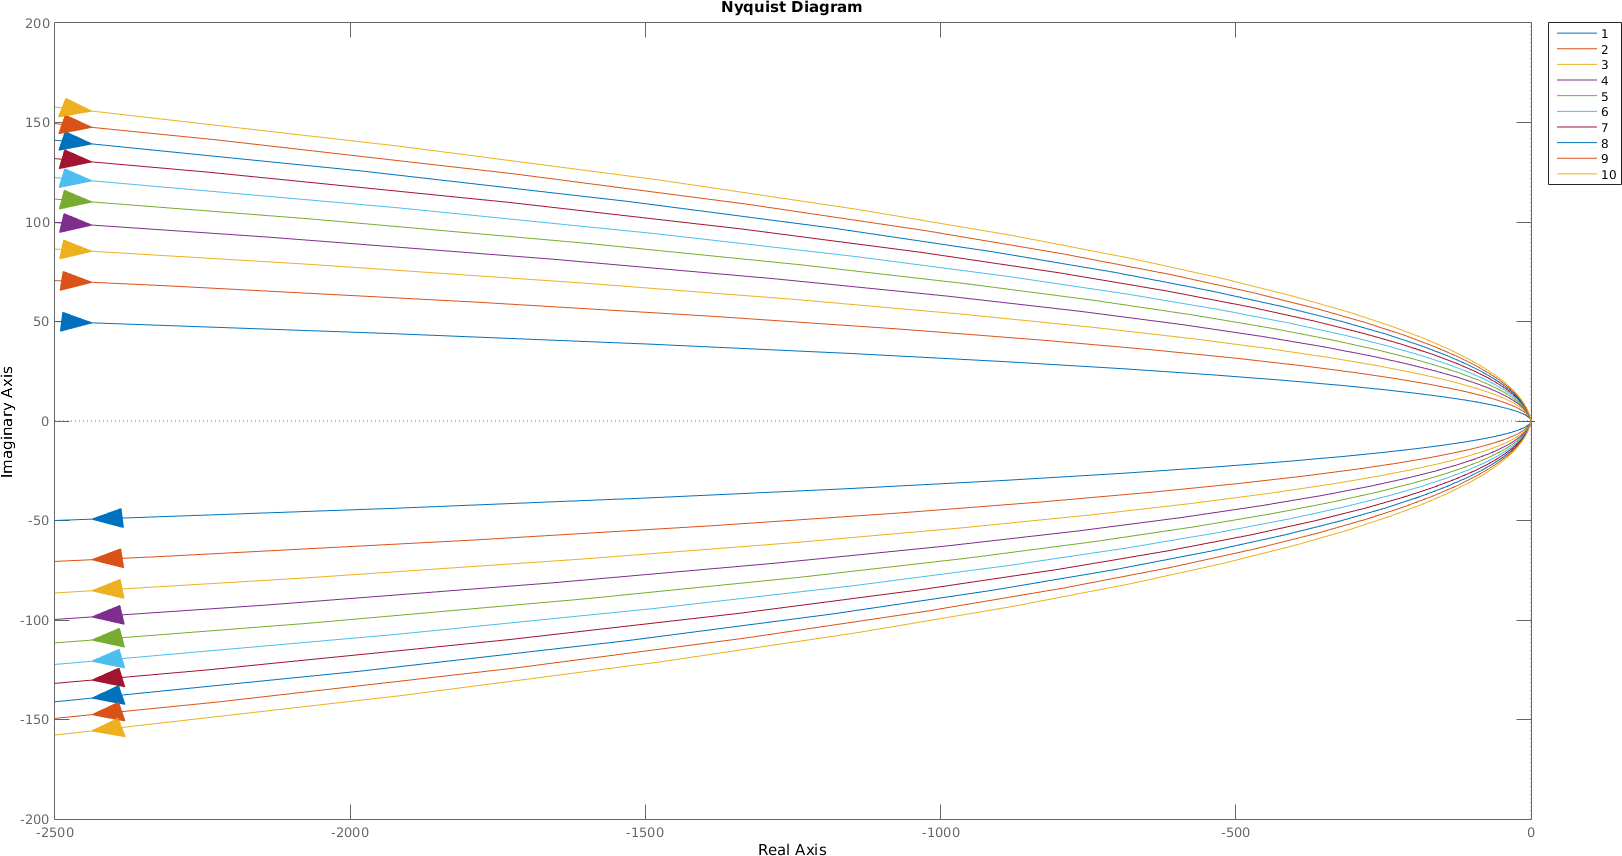
\includegraphics[scale=0.4]{nyquist1}
    \label{fig:nyquist1}
\end{figure}

Como pode ser observado na figura \ref{fig:nyquist1} (gerada a partir do código \ref{cod:nyquist1}), o valor de K não desloca o gráfico. Analisando a resposta ao degrau do sistema (figura \ref{fig:step1}), é possível observar o mesmo se mantem instável independente do valor de K.

\begin{figure}[H]
    \centering
    \caption{Resposta ao degrau para $ 1 \leq K \leq 10$.}
    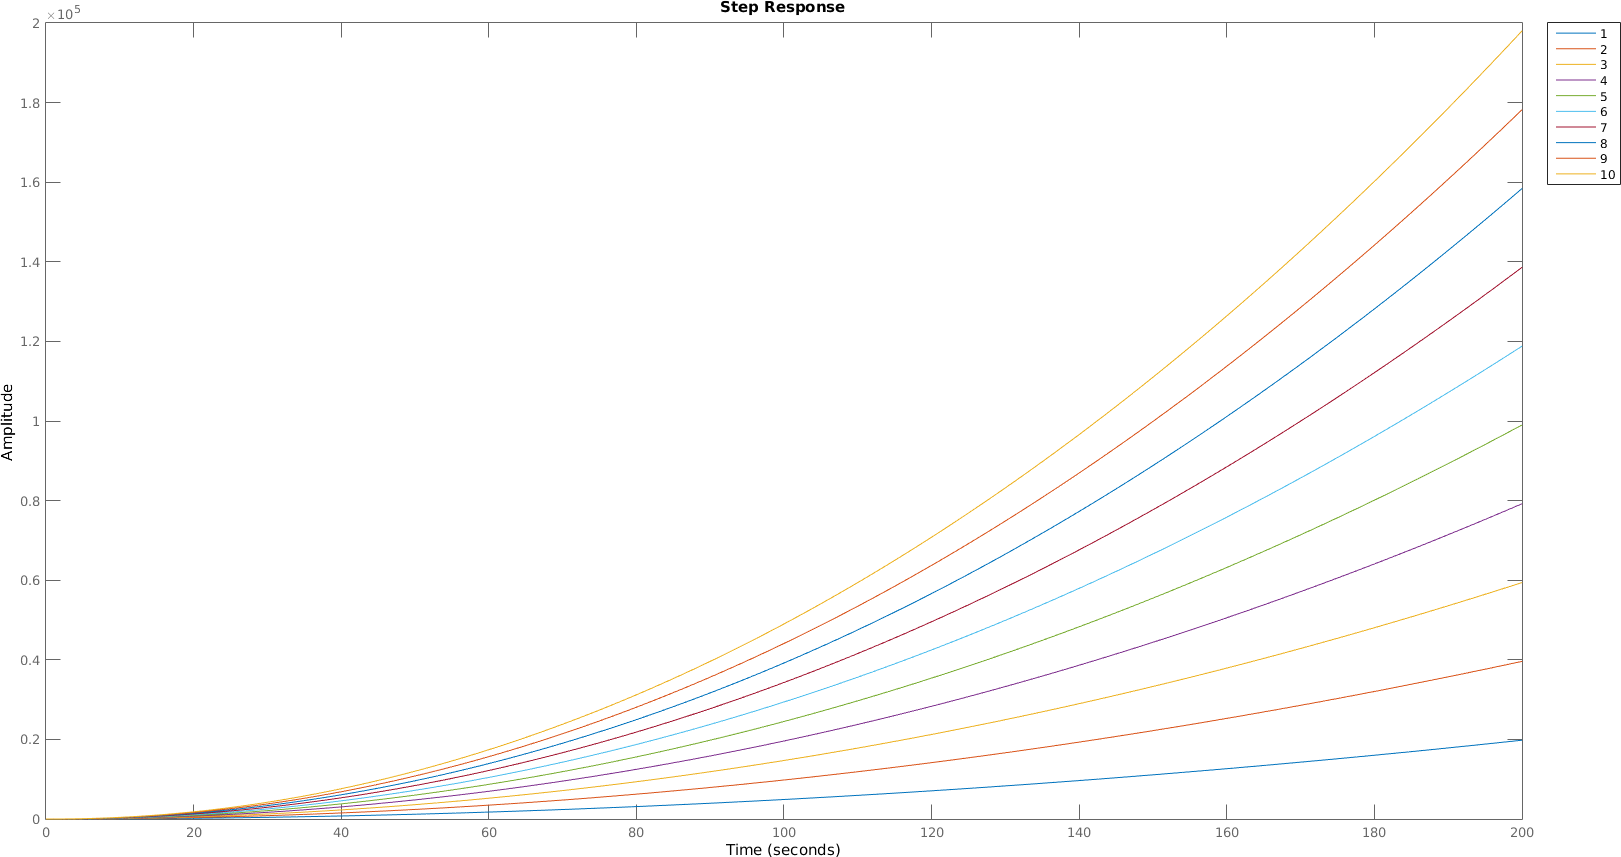
\includegraphics[scale=0.4]{step1}
    \label{fig:step1}
\end{figure}

\subsection*{Projeto do controlador}

Para $mp \leq 5 \, \%$, $\zeta \geq 0,7$ e para $t_s \leq 1 \, s$, $\omega_n \geq 4$ (aproximação de 2\%). Assim, os polos desejados são:

\[
    p = 6,3 \pm j6,3.
\]

O ângulo é:

\[
    \theta = tg^{-1} \left( \frac{6,3}{6,3} \right) \cong 45^\circ
\]

A contribuição angular do controlador é:
\[
    \beta = -180^\circ + 225^\circ = 45^\circ
\]

Devemos também adicionar um zero na origem, para poder utilizar o controlador de avanço de fase, assim, o controlador será:

\[
    C(s) = K_c s \left( \frac{s+4}{s+20} \right)
\]

O ganho $K_c$ foi determinado com o uso do recurso \emph{rctool} do matlab, sendo $K_c = 32.9$. A imagem \ref{fig:lead} mostra o \textit{root locus} do sistema, sendo que, a região em branco é a região que atende as especificações.

\begin{figure}[H]
    \centering
    \caption{\textit{Root Locus} para a planta $G(s)$ com o controlador $C(s)$.}
    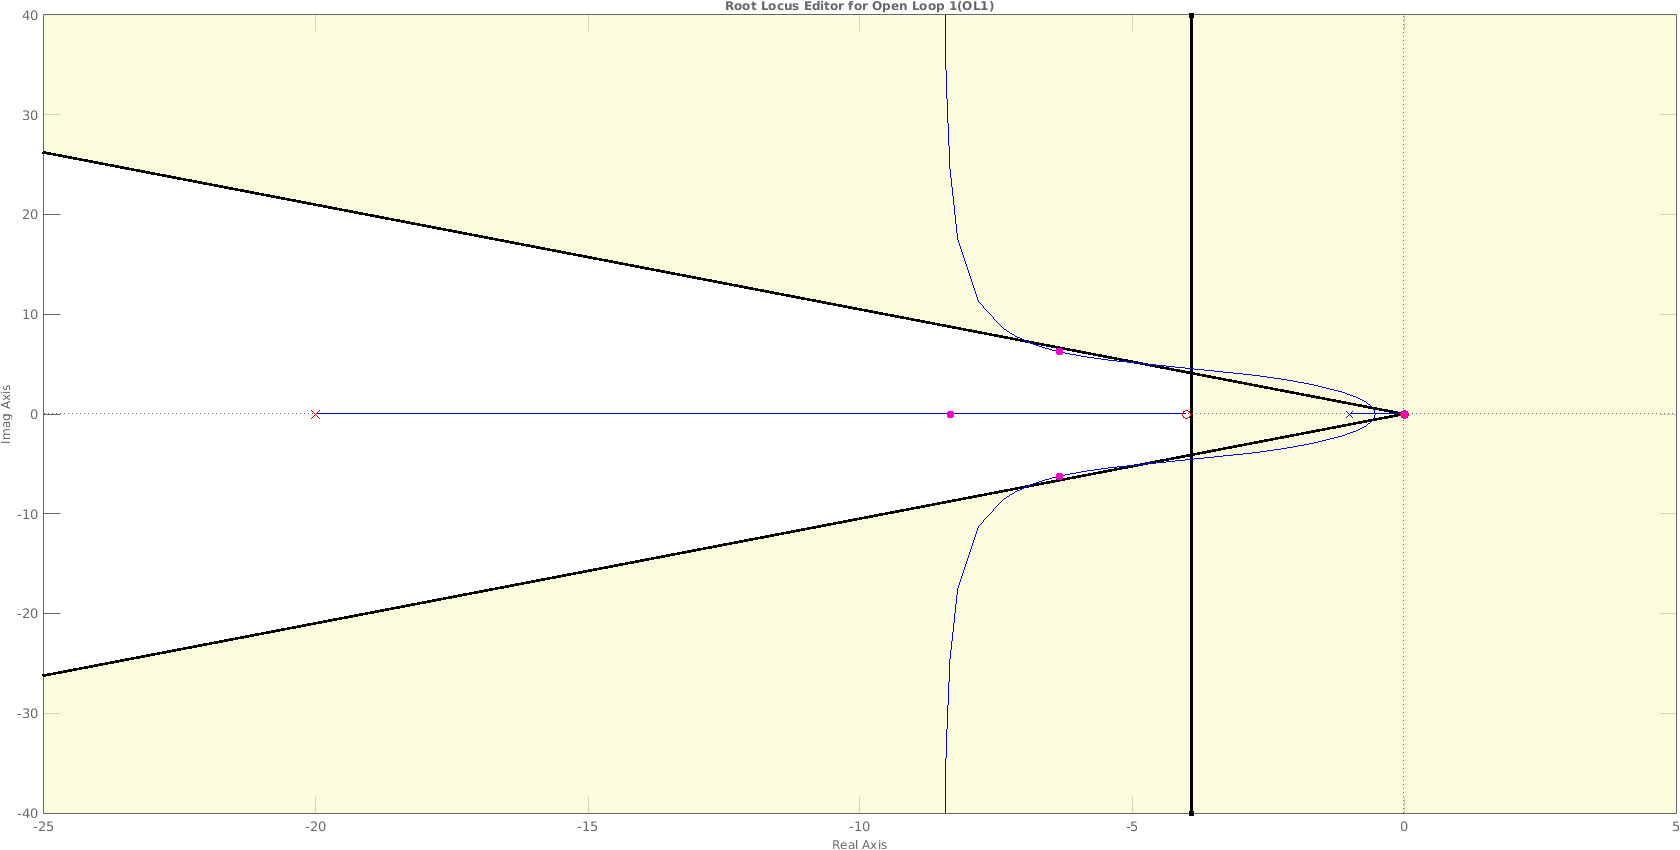
\includegraphics[scale=0.35]{lead}
    \label{fig:lead}
\end{figure}

\subsection*{Análise da estabilidade com o controlador}

Para confirmar a estabilidade do sistema, a figura \ref{fig:impulse} mostra que o sistema a resposta do sistema ao impulso unitário tende a zero e a figura \ref{fig:step2} mostra que o sistema é de fato estável para a entrada degrau.

\begin{figure}[H]
    \centering
    \caption{Resposta ao impulso do sistema.}
    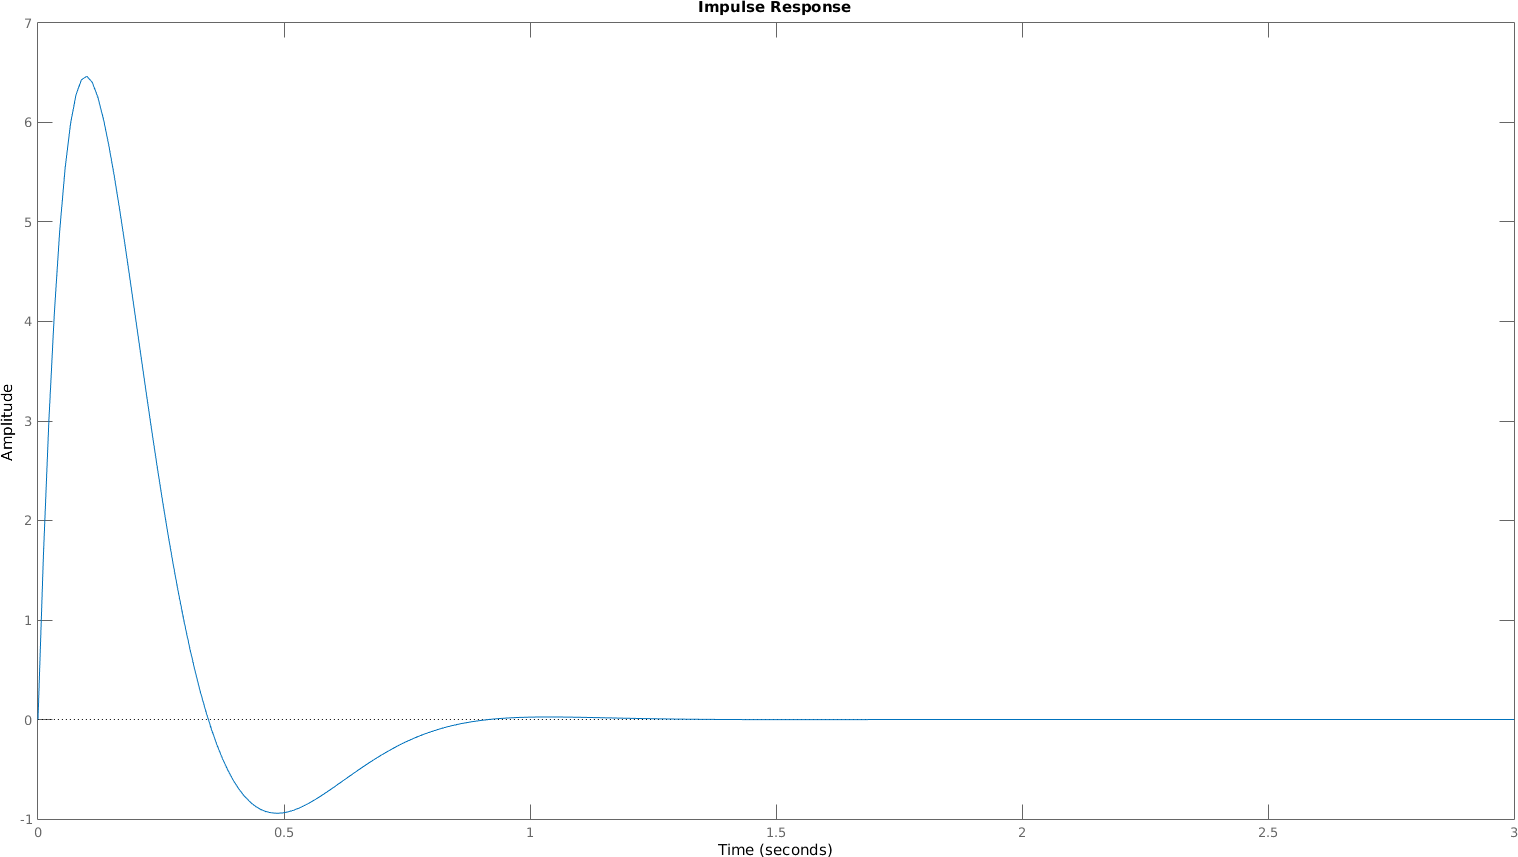
\includegraphics[scale=0.35]{impulse}
    \label{fig:impulse}
\end{figure}

\begin{figure}[H]
    \centering
    \caption{Resposta ao degrau do sistema.}
    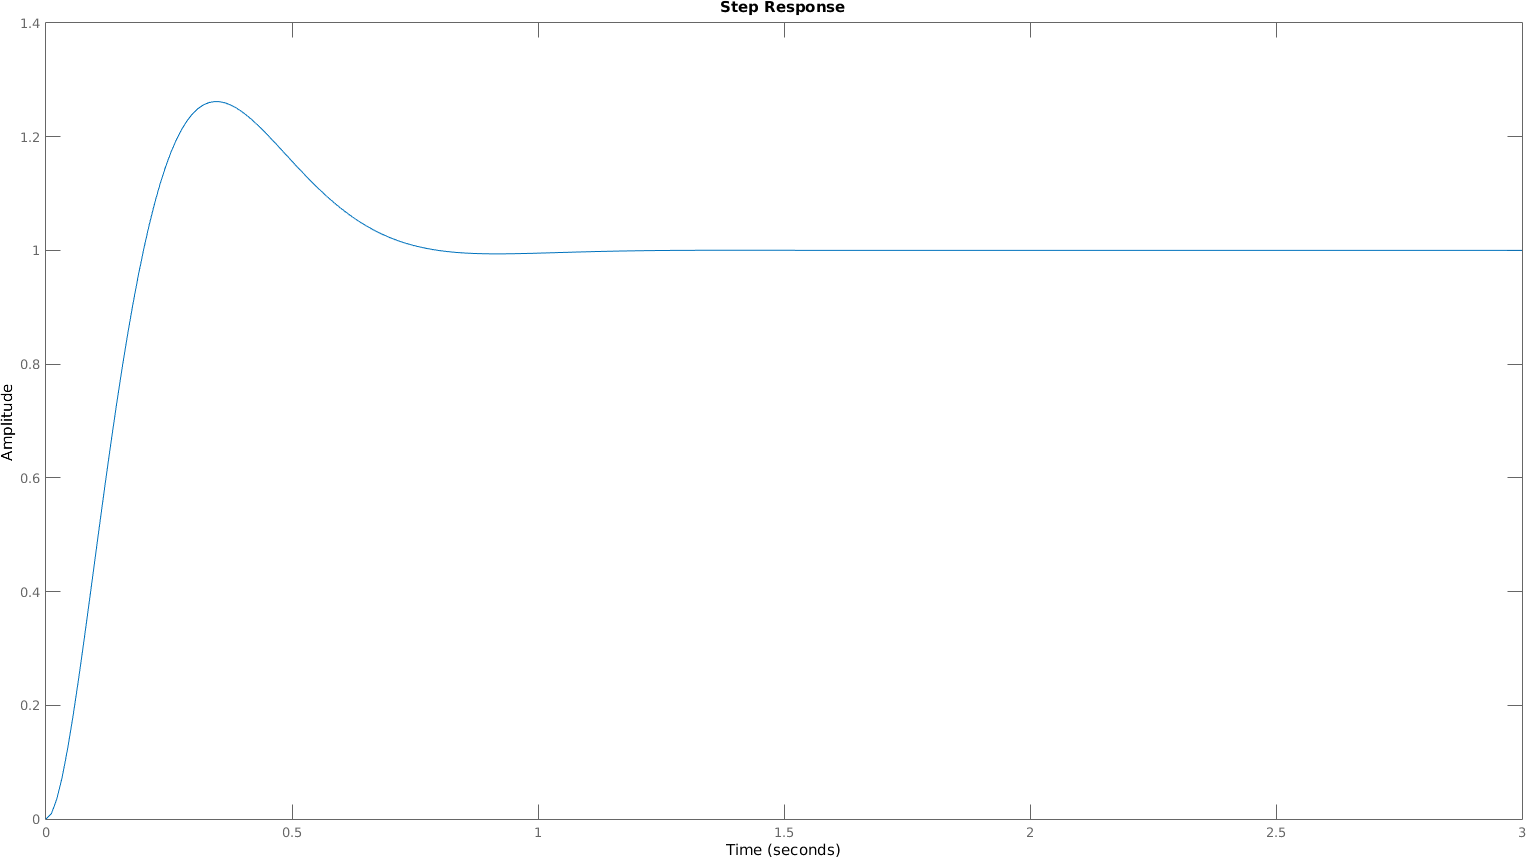
\includegraphics[scale=0.35]{step2}
    \label{fig:step2}
\end{figure}

Por ultimo, o diagrama de Nyquist, figura \ref{fig:nyquist2}, também mostra que o sistema é estável.

\begin{figure}[H]
    \centering
    \caption{Diagrama de Nyquist para o sistema.}
    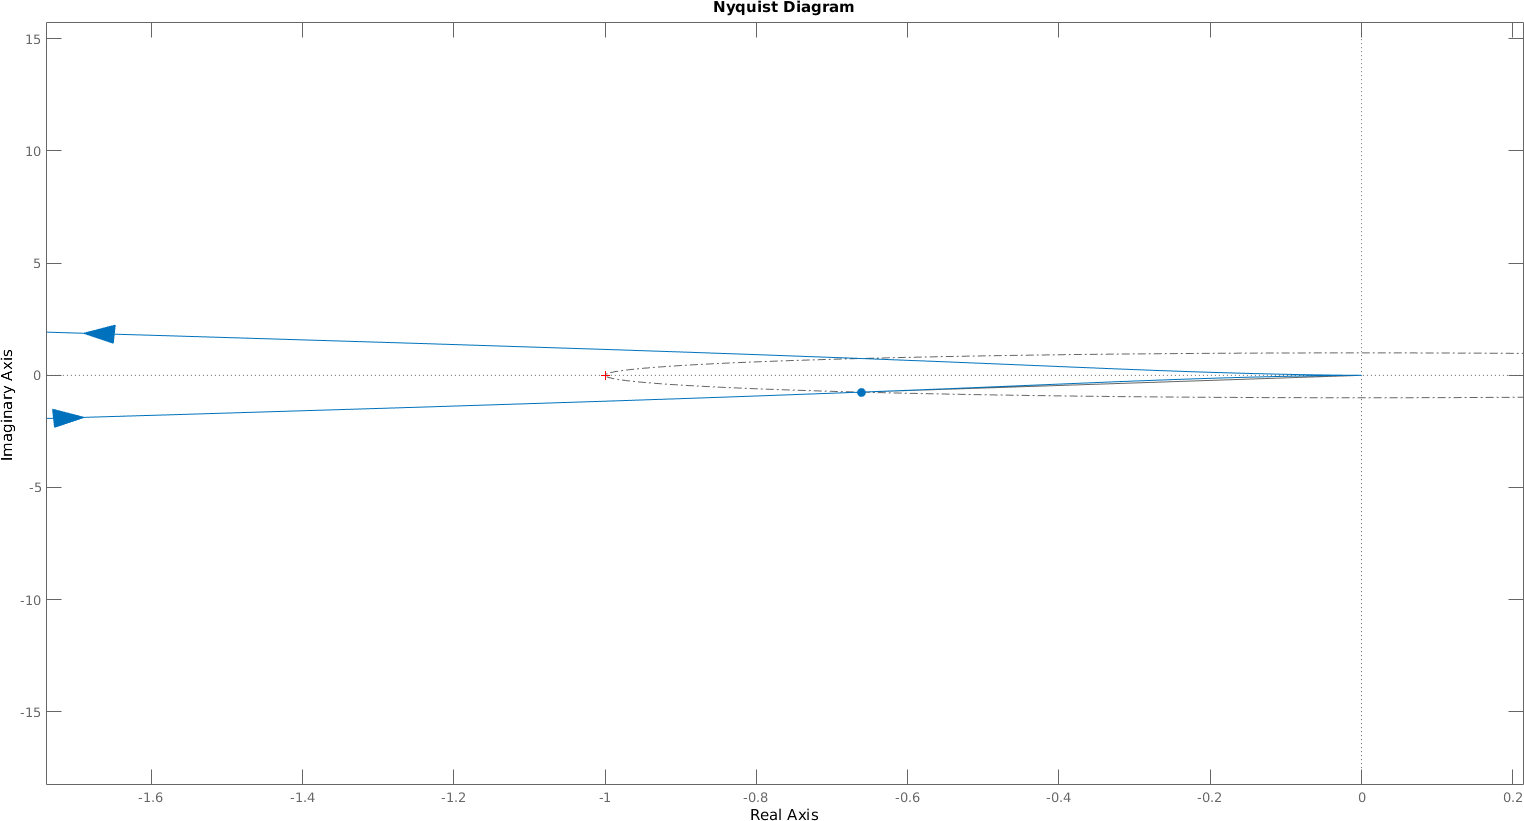
\includegraphics[scale=0.35]{nyquist2}
    \label{fig:nyquist2}
\end{figure}


\end{document}